=\newpage
\section{Set Theory}

\emph{Set theory} is a foundational branch of mathematics that studies \emph{sets}, which are simply 
collections of objects. At its core, it deals with the fundamental concepts of membership 
(whether an object belongs to a set), equality (when two sets are the same), and relationships 
between sets (like subsets, intersections, and unions).

It might seem simple, but set theory provides the basic language and tools to define 
and reason about almost all mathematical objects, from numbers and functions to 
more complex structures. It helps us understand the concept of infinity, organize mathematical 
ideas logically, and resolve paradoxes that arise from dealing with collections.

In essence, set theory provides the building blocks upon which much of modern mathematics is constructed.

Note, that I will start with sets as such instead of going through classes and then exporting some of their 
properties to sets. Classes will only be handled shortly with the axioms and some proofs but some of their properties will be 
directed presented as set properties. 

\subsection{Basics}

To be concise, a set is a collection of mathematical objects that can also be other sets.
Here is a list of common symbols for set theory.

\begin{itemize}

	\item \(A \subseteq B\): Set \(A\) is a subset of \(B\). This means every element of 
		  \(A\) is also in \(B\).

	\item \(A \subseteq B\) or \(A = B\): This notation already includes the possibility that \(A\) 
		  equals \(B\) since a set is always a subset of itself.

	\item \(A \cup B\): The union of sets \(A\) and \(B\). It includes all elements 
	      that are in \(A\), in \(B\), or in both.

	\item \(A \cap B = A \setminus (A \setminus B)\): The intersection of sets \(A\) and \(B\). It includes only the elements 
	      that are in both sets.

	\item \(A \setminus B\): The difference of sets. Elements in \(A\) that are not in \(B\).

	\item \(A^c\) or \(\overline{A}\): The complement of set \(A\). All elements not in \(A\), 
		  relative to  a universal set.

	\item \(|A|\): The cardinality of set \(A\), which is the number of elements in the set.

\end{itemize}

\subsubsection{Visuals}

\begin{figure}[H]
	\centering
	\begin{minipage}{0.45\textwidth}
		\centering
		
\begin{tikzpicture}[scale=0.8]
			% 1. Empty set
			\node at (0,0) {\textbf{1.} \(\emptyset\)};
			\draw (2,-0.5) circle (0.5);
		\end{tikzpicture}
		\caption*{1. Empty Set}
	\end{minipage}
	\hfill
	\begin{minipage}{0.45\textwidth}
		\centering
		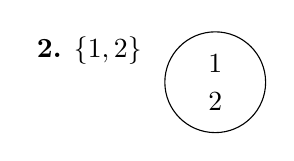
\begin{tikzpicture}[scale=0.8]
			% 2. Set with two elements
			\node at (0,0) {\textbf{2.} \(\{1,2\}\)};
			\draw (2,-0.5) circle (0.8);
			\node at (2,-0.2) {1};
			\node at (2,-0.8) {2};
		\end{tikzpicture}
		\caption*{2. Set with Two Elements}
	\end{minipage}

	\vspace{0.5cm}

	\begin{minipage}{0.45\textwidth}
		\centering
		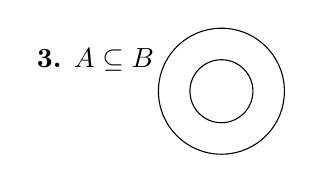
\begin{tikzpicture}[scale=0.8]
			% 3. A subset of B
			\node at (0,0) {\textbf{3.} \(A \subseteq B\)};
			\draw (2,-0.5) circle (1);
			\draw (2,-0.5) circle (0.5);
		\end{tikzpicture}
		\caption*{3. A is a subset of B}
	\end{minipage}
	\hfill
	\begin{minipage}{0.45\textwidth}
		\centering
		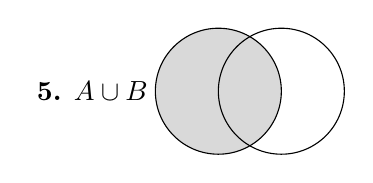
\begin{tikzpicture}[scale=0.8]
			% 5. Union
			\node at (0,0) {\textbf{5.} \(A \cup B\)};
			\begin{scope}
				\clip (2,0) circle(1);
				\fill[gray!30] (3,0) circle(1);
			\end{scope}
			\fill[gray!30] (2,0) circle(1);
			\draw (2,0) circle(1);
			\draw (3,0) circle(1);
		\end{tikzpicture}
		\caption*{5. Union of A and B}
	\end{minipage}

	\vspace{0.5cm}
\end{figure}

\newpage

\begin{figure}
	\centering
	\begin{minipage}{0.45\textwidth}
		\centering
		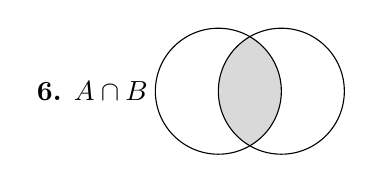
\begin{tikzpicture}[scale=0.8]
			% 6. Intersection
			\node at (0,0) {\textbf{6.} \(A \cap B\)};
			\begin{scope}
				\clip (2,0) circle(1);
				\fill[gray!30] (3,0) circle(1);
			\end{scope}
			\draw (2,0) circle(1);
			\draw (3,0) circle(1);
		\end{tikzpicture}
		\caption*{6. Intersection of A and B}
	\end{minipage}
	\hfill
	\begin{minipage}{0.45\textwidth}
		\centering
		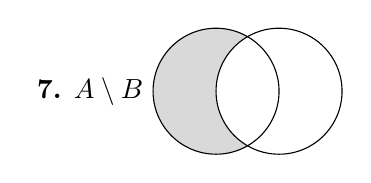
\begin{tikzpicture}[scale=0.8]
			% 7. A \ B
			\node at (0,0) {\textbf{7.} \(A \setminus B\)};
			\fill[gray!30] (2,0) circle(1);
			\begin{scope}
				\clip (3,0) circle(1);
				\fill[white] (2,0) circle(1);
			\end{scope}
			\draw (2,0) circle(1);
			\draw (3,0) circle(1);
		\end{tikzpicture}
		\caption*{7. A minus B}
	\end{minipage}

	\vspace{0.5cm}

	\begin{minipage}{0.45\textwidth}
		\centering
		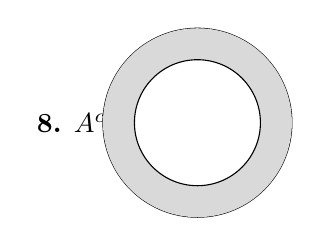
\begin{tikzpicture}[scale=0.8]
			% 8. Complement
			\node at (0,0) {\textbf{8.} \(A^c\)};
			\draw (2,0) circle(1.5);
			\fill[gray!30] (2,0) circle(1.5);
			\fill[white] (2,0) circle(1);
			\draw (2,0) circle(1);
		\end{tikzpicture}
		\caption*{8. Complement of A}
	\end{minipage}
\end{figure}
\smallskip

\subsection*{Short History Lesson}

When set theory was invented back then by Cantor, he had no formal axioms but a set of basic 'common sense' rules he assumed when 
creating his theory. This choice lead to a famous paradox known as \emph{Russell's Paradox}. The paradox states that: "Given a set S which is 
the set containing all sets which do not contain themselves. The S does not contain itself, but if it does not contain itself it must contain itself". 
In short \(S = \{x: x \notin x\}\), this is a so-called \emph{logical} paradox. This is of course a huge contradiction in the hearth of naive set theory. The choice to take a more 
formal and axiomatic approach was to eliminate such fundamental faults.

As a short teasing we will declare the \emph{Axiom of Selection:} \(\{x \in A: S(x)\}\) this means that we can construct a set of elements 
of an existing set as long as they satisfy a condition. Now the paradox of \(x: x \notin x\) can not be state directly in our new system. We can emulate it by 
declaring 

\[	
	S = \{x \in A \mid x \notin x\}
\]

By analyzing the expression we get that, if \(S \notin S\) then \(S \in S \land S \in A\) which will be a contradiction, 
therefore, \(S \notin A\).

Continuing this small historic section, we will also need to limit the power of our condition of statements \(S(x)\) to get rid of another type 
of paradoxes considered as \emph{semantic}.

For example, we could define the following set:

\[
	\{x \in \N : \text{ x can be described in less than 20 words of the English language}\}
\]

Note that this set would need to be finite because it there is only a limited amount of combination of words in the English language. But we could 
for example say: 'the natural number which can not be described in less than 20 words' this number. This is again an example of an element in 
a set if and only if it is not in the set. To formalize our conditions we 

\subsection{Sets and Classes}

One important distinction is the system of Neumann is notion difference between a \emph{set} and \emph{class}.
Classes can not be contained inside sets, while sets can. Formally:

If \(X \in Y\) for some class \(Y\) then \(X\) is a set. If \(X \notin Y\) for any class \(Y\) then \(X\) is a class.

\subsection{Axioms of Set Theory}

\begin{enumerate}[label = \Roman*.]
	
	\item \emph{Axiom of Selection}: Given a class \(A\), a class \(S\) can be build in the following manner \(S = \{x \in A \mid P(x)\}\)
	 
	\item \emph{Axiom of Equality}: Let \(A\) and \(B\) be classes then \(A = B \iff \forall X : A \in X \implies B \in X \land B \in X \implies A \in X\)

	\item \emph{Empty-Set Axiom}: \(\emptyset\) is a set. 
	
	\item \emph{Axiom of Class Construction}: Let \(P(x)\) be a statement about \(x\) which can be expressed in terms of \(\in, \land, \lor ,\neg, \implies, \exists, \forall \) 
	with variables \(x,y,z,\dots\) then there exists a class \(C\) whose elements consist of all the elements \(x\) which satisfy \(P(x)\). \(\{x : P(x)\}\)
	
	\item \emph{Axiom of Subset}: Every subclass of a set is a set.

	\item \emph{Axiom of Paring}: Is \(a\) and \(b\) are sets, then \(\{a, b\}\) is a set

	\item \emph{Axiom of Union}: If \(A\) is a set of sets, then \(\bigcup_{a \in A} a\) is a set.

	\item \emph{Axiom of the Power Set}: If \(A\) is a set then the set of all the subsets of the original set, \(\mathcal{P}(A)\), is a set.

	\item \emph{Axiom of Foundation}: If \(A\) is any set, there is an element \(a \in A\) such that \(a \cap A = \emptyset\). Alternatively, there exists not such set, 
	which is formed from a chain like: \(a_1 \in a_2 \in a_3 \in \dots\). \(\forall S(S \neq \emptyset \implies \exists x \in S \forall y \in S y \notin x)\)

	\item \emph{Axiom of Replacement}: If \(A\) is a set and \(f: A \to B\) is a surjective function, then \(B\) is a set.

	\item \emph{Axiom of Infinity}: An infinity set exists.

	\item \emph{Axiom of Choice}: 

\end{enumerate}

\subsubsection*{Proofs Using the Axioms}

\begin{itemize}

	\item \(A = A\) and also \(A = B \implies B = A\): The statements is trivial by the first axiom 

	\item \(A \subseteq B \land B \subseteq A \implies A = B\): \((\forall x \in A \implies x \in B) \land (\forall x \in B \implies x \in A)\) Let us 
	suppose for the sake of contradiction that \(A \neq B\) then \(\exists x \in A: x \notin B\) or the other way around. Note that this statement contradicts our 
	initial conditions. Thus, the statement is true.

	\item \(A \subseteq B \land B \subseteq C \implies A \subseteq C\): \((\forall x \in A \implies x \in B) \land (\forall x \in B \implies x \in C)\) By a similar manner 
	let us assume that \(A\) is not a subset of \(C\) this means that for some \(x\) the condition holds that \(x \in A \land x \notin B\) because else it would be in \(C\). 
	Note that because \(A \subseteq B\) such an \(x\) can not exist due to our initial condition and also \(B \subseteq A\) for that case. Thus \(A \subseteq C\)

	\item \(\emptyset \subseteq A\): By definition \(x \in \emptyset \implies x \in A\), by contrapositive \(x \notin A \implies x notint \emptyset\). This is true 
	because of the contrapositive being true.

	\item Given a proper class \(A \subseteq B\) prove that \(B\) is a proper class and that the union of two proper classes is also a proper class. 
	
	Given \(A \subseteq B\), if \(B\) would be not be a proper class then by the property which states that every subclass of a class 
	is a set we would have a contradiction. Therefore, \(B\) is a proper class.

	\(A \cap C\) were \(A\) and \(C\) are proper classes, gives us that their union is also a proper class due to \(A, C \subseteq A \cup C\)

	\item \(\mathcal{P}(A) \nsubseteq A\): Let \(x \in \mathcal{P}(a)\), then \(\forall x \in \mathcal{P}(A) \implies x \in A\). By definition, \(A \in \mathcal{P}(A)\), but 
	\(A \notin A\); hence we have contradiction and the power set of a set is not a subset of the original set.
	 
\end{itemize}

\QED 

\subsection{Consequences of the Axiom of Replacement}

\begin{itemize}
	
	\item Every singleton is a set. 

	\item If \(A\) is in a one-to-one correspondence with \(B\), then \(B\) is a set.
	
	\item If \(\{A_i\}_{i \in I}\) is an indexed family of sets and \(I\) is a set, then \(\{A_i \mid i \in I\}\) is a set.

\end{itemize}

\subsection{Subclasses/Subsets}

A subset/subclass \(A\) of the set/class \(B\) is a set which obeys the following property:

\[
	A \subseteq B \iff \forall x \in A, x \in A \implies x \in B
\]

\subsection{The Universal Class}

By the axiom of construction we define \(\mathcal{U}\) with \(P(x)\) is \(x = x\) as the \emph{universal class} of all elements.

It also as the following property

\[
	A \subseteq \mathcal{U},
\]

which gives us the following: \(A \cup \mathcal{U} = \mathcal{U}\) and \(A \cap \mathcal{U} = A\) for any class or set \(A\).

\subsection{The Empty Class}

The \emph{empty class} is class with no elements. 

\[
	\emptyset = \{x \mid x \neq x\}
\]

We can not use existence quantifiers \(\exists\) with this class.
Every statement with \(\forall x \in \emptyset\) is true, because there are no counterexamples. 
This leads to interesting equalities like \(\mathcal{U} = \emptyset\).

We can prove that the empty class exist by letting \(\emptyset = \{x \mid x \ne x\}\) this is a perfectly valid statement.

Now we need to prove that it is unique, and this is given by the axiom of extensionality.

\QED

\subsection{The Empty Set}

The set that contains no elements \(\emptyset\). It is the unique set with 
zero elements. It inherits the properties of its class counterpart.

It also has the property that \(\emptyset \subseteq A\) for any class or set \(A\).

\subsection{Set Complement Proof}

Given \(A, B \subseteq M\) then \(A \subseteq B \implies B^c \subseteq A^c\)

For some \(x \in B^c\) we know that \(x \notin B\). If \(x \in A\) then \(x \in B\) which is a contradiction. 
Hence, \(x \notin A\) therefore, for every \(x \in B^c\) we conclude \(B^c \subseteq A^c\).

\QED

\subsection{Proof The Power Set of a Set is not an Element of the Set}

Let \(X\) be a set and \(Y = \{x \in X \mid x \notin x\}\). 

This is a subset of \(X\) by definition and implies \(Y \in \mathcal{P}(X)\). 

Assume \(\mathcal{P}(X) \subseteq X\) then \(Y \subseteq X, Y \in X\) but 

\[
	Y \in Y \implies Y \notin Y \implies Y \in Y \text{ which is a contradiction}
\]

Because our assumption was proven false, then \(\mathcal{P}(X)\) is not a subset of \(X\).

\QED 

\subsection{Proof of the Union of Subsets}

Let \(A\) and \(B\) be sets then: 

\begin{itemize}

    \item \(A \subseteq B\) if and only if \(A \cup B = B\)
	
	\item \(A \subseteq B\) if and only if \(A \cap B = A\)

\end{itemize}

\textbf{Proof:}

For \(A \subseteq B \iff A \cup B = B\) we know that \(x \in A \implies x \in B \) Then

\begin{align*}
	A \cup B &\iff x \in A \lor x \in B \quad \text{ as subset then } \\ 	
	&\iff x \in B \lor x \in B \\ 
	&\iff x \in B = B
\end{align*}

The other direction will be skipped due to it being very similar to the \(\Rightarrow\) direction. 

Similarly, for \(A \subseteq B \iff A \cap B = A\) We know that for some \((y \in B \land y \notin A) \notin A \cap B\) because of 
the definition of the subset. Then this tells us that \(\forall x \in A \cap B: x \in A\) thus \(A \cap B = A\)

\QED

\subsubsection*{Cut of Set and Complement}

\(A \cap B^c = \emptyset \iff A \subseteq B\)

\(\Rightarrow\):

\begin{align*}
	A \cap B^c = \emptyset &\implies \nexists x \in A \land x \nexists x \in B^c \\ 
	&\implies \forall x \in A: x \in B \\ 
	&\iff A \subseteq B
\end{align*}

\(\Leftarrow:\) Let us assume that \(A\) is not a subset of \(B\) then

\begin{align*}
	\exists x \in A \land x \notin B &\implies x \in A \land x \in B^c \\ 
	&\implies x \in A \cap B^c \implies A \cap B^c \neq \emptyset
\end{align*}

\QED 

\subsection{The Singleton and Doubleton}

We define the \emph{singleton} as 

\[
	\{a\} := \{x \mid x = a\},
\]

and the \emph{doubleton} as

\[
	\{a, b\} := \{x \mid x = a \lor x = b\},
\]

\subsubsection*{Properties}

\begin{itemize}

	\item \(\{a\} = \{b\} \iff a = b\)
	
	\item \(\{a, b\} = \{a\} \iff a = b\)

	\item \(\{a, b\} = \{x, y\} \iff (a = x \land b = y) \lor (a = y \land b = x)\)

\end{itemize}

\textbf{Proofs:}

\(\{a\} = \{b\} \iff a = b\), by the axiom of the equality of sets if 

\[
	\exists x \in \{a\}: x \notin \{b\} \implies \{a\} \neq \{b\},
\]

which is a contradiction to our condition thus \(a = b\). Similarly, we can use the same argument for the other 
direction of the proof.

\QED 

\(\{a, b\} = \{a\} \iff a = b\) can be proven using the definition and the equivalence \(P \lor P = P\)

\[
	\{a, b\} := \{x \mid x = a \lor x = a\} \implies \{x \mid x = a\}
\]

\QED

\(\{a, b\} = \{x, y\} \iff (a = x \land b = y) \lor (a = y \land b = x)\), we need to first the case \(a = b\). In 
that case our problems simplifies to \(\{a\} = \{x, y\}\) which by the axiom guarantees the equality for \(\{a\} = \{x\} \lor \{a\} = \{y\}\) 
because otherwise we will arrive at a contradiction.

For the case \(a \neq b\) we have the following cases \((x = a \land y = b) \lor (x = b \land y = a)\) which against by the use of the axiom of 
the equality we can discard the cases where the equality does not hold.

\QED

\subsection{Ordered Pair}

Let \(A\) and \(B\) be two non-empty sets and \(m \in A, n \in B\). We define 

\[
	(m,n) := \{\{m, n\}, {m}\}	
\]

and 

\[
	(n,m) := \{\{m, n\}, {n}\}	
\]

as ordered pairs which are elements of \(A \times B\) and \(B \times A\) respectively.

\subsection{The Cartesian Product}

The Cartesian product of two sets \(A\) and \(B\), written \(A \times B\), is the set of 
all ordered pairs in which the first element belongs to \(A\) and the second belongs to \(B\):

\[
	A \times B = \{ (a, b) : a \in A, \land\ b \in B\}
\]

\textbf{Example:}

\begin{table}[H]
	\centering
	\caption{Cartesian Product of \(A = \{1, 2, 3\}\) and \(B = \{4, 5, 6\}\)}
	\begin{tabular}{|c|c|c|c|}
		\hline
		\multirow{3}{*}{\(A \times B\)} & \multicolumn{3}{c|}{\(b \in B\)}                       \\
		\cline{2-4}
		                              & \(4\)                            & \(5\)      & \(6\)      \\
		\hline
		\(a \in A\)                     &                                &          &          \\
		\hline
		\(1\)                           & \((1, 4)\)                       & \((1, 5)\) & \((1, 6)\) \\
		\hline
		\(2\)                           & \((2, 4)\)                       & \((2, 5)\) & \((2, 6)\) \\
		\hline
		\(3\)                           & \((3, 4)\)                       & \((3, 5)\) & \((3, 6)\) \\
		\hline
	\end{tabular}
	\label{tab:cartesian_product}
\end{table}

The general Cartesian product of \(n\) sets can be written as:

\begin{align*}
	X_{i = 1}^{n + 1} A_i & = \left( X_{i = 1}^{n} A_i \right) \times A_{n + 1} \quad \text{with} \quad X_{i = 1}^{1} A_i = A_1 \\
	\text{When } A_i      & = M \ \text{for all } i:                                                                            \\
	M^n                   & := M \times M \times \cdots \times M = X_{i = 1}^{n} M \quad \text{with} \quad M^1 = M
\end{align*}

\subsubsection*{Distributive Law for the Cartesian Product}

Let \(A, A' \subseteq X\) and \(B, B' \subseteq Y\). Then

\[
	(A \times B) \cap (A' \times B') = (A \cap A') \times (B \cap B').
\]

We prove the equality by showing both inclusions.

1. Direction: \((A \times B) \cap (A' \times B') \subseteq (A \cap A') \times (B \cap B')\).

\begin{align*}
	&\text{Let } (x,y) \in (A \times B) \cap (A' \times B'). \\
	&\iff (x,y) \in A \times B \text{ and } (x,y) \in A' \times B' \\
	&\iff x \in A,\, y \in B \text{ and } x \in A',\, y \in B' \\
	&\iff x \in A \cap A' \text{ and } y \in B \cap B' \\
	&\iff (x,y) \in (A \cap A') \times (B \cap B').
\end{align*}

2. Direction: \((A \cap A') \times (B \cap B') \subseteq (A \times B) \cap (A' \times B')\).

\begin{align*}
	&\text{Let } (x,y) \in (A \cap A') \times (B \cap B'). \\
	&\iff x \in A \cap A' \text{ and } y \in B \cap B' \\
	&\iff x \in A,\, x \in A' \text{ and } y \in B,\, y \in B' \\
	&\iff (x,y) \in A \times B \text{ and } (x,y) \in A' \times B' \\
	&\iff (x,y) \in (A \times B) \cap (A' \times B').
\end{align*}

Thus, both inclusions hold and the equality follows.

\QED 

\subsubsection*{Proof that the Cartesian Product is a Set}

We need to prove that \(A \times B \subseteq \mathcal{P}(A \cup B)\). By the definition of the ordered pair we know that 
for \(x \in A \cup B \implies \{x\} \subseteq A \cup B\) the same for \(x,y \in A \cup B\) which implies 
\(\{x, y\} \subseteq A \cup B\). By our axiom of union we know that \(\{\{x\}, \{x, y\}\}\) is a set a and this is a 
subset of \(\mathcal{P}(\mathcal{P}(A \cup B))\) for free \(x\) and \(y\). Hence 

\[
	(x, y) \subseteq A \times B \subseteq \mathcal{P}(\mathcal{P}(A \cup B))
\]

\QED

\subsubsection*{Proof the empty set of the Cartesian Product}

\(A \times B = \emptyset \iff A = \emptyset \lor B = \emptyset\). We will prove the negation of the 
statement which logically equivalent.

\[
	A \times B \ne \emptyset \iff A \neq \emptyset \land B \neq \emptyset
\]

\(\Rightarrow\): 

\begin{align*}
		A \times B \ne \emptyset &\implies \exists (x,y) \in A \times B: x \in A \land y \in B \\ 
		&\implies \exists x \in A \land \exists y \in B \\ 
		&\implies A \neq \emptyset \land B \neq \emptyset
\end{align*}


\(\Leftarrow\):

\begin{align*}
	A \neq \emptyset \land B \neq \emptyset &\implies\exists x \in A \land \exists y \in B \\ 
	&\implies A \times B \neq \emptyset
\end{align*}

\QED 

\subsection{Laws of Set Algebra}

Let \(X\) be the universal set and \(A, B, C \subseteq X\).

\begin{itemize}
	
	\item \(\emptyset \subseteq A\)
	
	\item \(A \subseteq B \iff A \cap B = A \iff A \cup B = B \iff X \setminus B \subseteq X 
		  \setminus A \iff B \subseteq A\)
	
	\item \(A \cup B = B \cup A\) 
	
	\item \(A \cap B = B \cap A\) 
	
	\item \((A \cup B) \cup C = A \cup (B \cup C)\) 
	
	\item \((A \cap B) \cap C = A \cap (B \cap C)\) 
	
	\item \(A \cap (B \cup C) = (A \cap B) \cup (A \cap C)\) 
	
	\item \(A \cup (B \cap C) = (A \cup B) \cap (A \cup C)\) 
		
	\item \(A \cup A = A \quad \text{and} \quad A \cap A = A\)
	
	\item \(A \setminus B = A \cap (X \setminus B) = A \cap \overline{B}\)
	
	\item \(B = \overline{A} \iff (A \cup B = X \land A \cap B = \emptyset)\) 
	
	\item \(\overline{A} \cap \overline{B} = \overline{A \cup B}\) 
	
	\item \(\overline{A} \cup \overline{B} = \overline{A \cap B}\) 
	
	\item \(\overline{\overline{A}} = A\)

	\item \((A \setminus B) \cup (B \setminus) A = A \Delta B\)

	\item \(A \setminus (B \cup C) = (A \setminus B) \cap (A \setminus C) \)
	
	\item \(A \setminus (B \cap C) = (A \setminus B) \cup (A \setminus C) \)

\end{itemize}

\subsubsection*{Proof of the Distributive Law}

\begin{align*}
	&\text{Let } x \in A \cap (B \cup C). \\
	&\iff x \in A \text{ and } x \in B \cup C \\
	&\iff x \in A \text{ and } (x \in B \text{ or } x \in C) \\
	&\iff (x \in A \text{ and } x \in B) \text{ or } (x \in A \text{ and } x \in C) \\
	&\iff x \in A \cap B \text{ or } x \in A \cap C \\
	&\iff x \in (A \cap B) \cup (A \cap C).
\end{align*}

Thus,

\[
	A \cap (B \cup C) \subseteq (A \cap B) \cup (A \cap C).
\]

\begin{align*}
	&\text{Conversely, let } x \in (A \cap B) \cup (A \cap C). \\
	&\iff x \in A \cap B \text{ or } x \in A \cap C \\
	&\iff (x \in A \text{ and } x \in B) \text{ or } (x \in A \text{ and } x \in C) \\
	&\iff x \in A \text{ and } (x \in B \text{ or } x \in C) \\
	&\iff x \in A \text{ and } x \in B \cup C \\
	&\iff x \in A \cap (B \cup C).
\end{align*}

Thus,
\[
	(A \cap B) \cup (A \cap C) \subseteq A \cap (B \cup C).
\]

\QED

\subsection{Proof of De Morgans's Law for sets and logic}

The complement of \( A \cup B \) is \( \overline{(A \cup B)} \), and the law on disjoint decomposition 
states:

\[
	B = \overline{A} \iff (A \cup B = X) \land (A \cap B = \emptyset)
\]

So define \( \overline{C} := A \cup B \) and \( D := \overline{A} \cap \overline{B} \),
and use Law (11) to show the disjoint decomposition:

\[
	D = C \iff A \cap B = A \cup B
\]

To show:

\[
	D \cup C = X \iff (\overline{A} \cap \overline{B}) \cup (A \cup B) = X
\]

\begin{align*}
	(\overline{A} \cap \overline{B}) \cup (A \cup B)
	 & = (\overline{A} \cup A \cup B) \cap (\overline{B} \cup A \cup B) \quad \text{(Law (8))} \\
	 & = (X \cup B) \cap (X \cup A)                                                            \\
	 & = X \cap X                                                                              \\
	 & = X
\end{align*}

To show:

\[
	D \cap C = \emptyset \iff (\overline{A} \cap \overline{B}) \cap (A \cup B) = \emptyset
\]

\begin{align*}
	(\overline{A} \cap \overline{B}) \cap (A \cup B)
	 & = (A \cap B \cap A) \cup (A \cap B \cap B) \quad \text{(Law (7))}                      \\
	 & = (\overline{A} \cap A \cap \overline{B}) \cup (\overline{A} \cap \overline{B} \cap B) \\
	 & = (\emptyset \cap \overline{B}) \cup (\overline{A} \cap \emptyset)                     \\
	 & = \emptyset \cup \emptyset                                                             \\
	 & = \emptyset
\end{align*}

\QED


\subsection{Indexed Sets}

Let \(X\) be a set, and \( A_i \subseteq X \) for all \( i \in J \), where \(I\) is the 
\emph{index set}.

If \( I = \{1, 2, \dots, n\} \) then we define 

\[
	\{A_i\}_{i \in I},
\]

as the set of all classes/sets for which an index in \(I\) exists.

We also can define the graph of the sets with their respective indexes:

\[
	G_{A_i} = A_i \times I = \{(i, A_i) \mid i \in I \land  A_i \in \{A_i\}_{i \in I}\}
\]

\subsection{Generalized Union, Intersection and Cartesian Product for Indexed Sets}

For a class of classes or sets of sets with an index set \(I\) we define the generalized \emph{union}, \emph{intersection} and \emph{Cartesian product} as:

\[
	\bigcup_{i=1}^{n} A_i := A_1 \cup A_2 \cup \dots \cup A_n = \{ x \mid \exists i \in I, (x \in A_i) \}
\]

\[
	\bigcap_{i=1}^{n} A_i := A_1 \cap A_2 \cap \dots \cap A_n = \{ x \mid \forall i \in I, (x \in A_i) \}
\]

\[
	X_{i=1}^{n} A_i = \{(a_1, \dots, a_n) \mid a_i \in A_i \}
\]

\subsection{Pairwise Disjoint}

If \(I\) is any set, then \( {(A_i)}_{i \in I} \) are \emph{pairwise disjoint} if and only if:

\[
	\forall i_1, i_2 \in I, \ i_1 \neq i_2 \implies A_{i_1} \cap A_{i_2} = \emptyset
\]

\subsection{Disjoint Decomposition}

If \(I\) is any set, then \( {(A_i)}_{i \in I} \) forms a \emph{disjoint decomposition} of \(X\) if 
and only if:

\[
	{(A_i)}_{i \in J} \text{ are pairwise disjoint and } \bigcup_{i \in J} A_i = X
\]

\subsection{Cardinality Laws}

Let \( A_i, B_j \subseteq X \) for \( i \in I \) and \( j \in J \). Then the following holds:

\begin{itemize}

	\item\emph{De Morgan's Laws:}

	\[
		\overline{\bigcap_{i \in I} A_i}= \bigcup_{i \in I} \overline{A_i} \quad \text{and} \quad 
		\overline{\bigcup_{i \in I} A_i} = \bigcap_{i \in I} \overline{A_i}
	\]

	\item \emph{Generalized Distributive Laws:}
	\[
		\left(\bigcap_{i \in I} A_i \right)\cup \left(\bigcap_{j \in J} B_j \right)= \bigcap_{i,j} (A_i \cup B_j) \quad \text{with} 
		\quad \bigcap_{i,j} = \bigcap_{(i,j) \in I \times J}
	\]

	\[
		\left(\bigcup_{i \in I} A_i \right) \cap \left(\bigcup_{j \in J} B_j \right) = \bigcup_{i,j} (A_i \cap B_j) \quad \text{with} 
		\quad \bigcup_{i,j} = \bigcup_{(i,j) \in I \times J}
	\]

\end{itemize}

Here, \( I = \{ 1, 2, 3, \dots, n \} \) and \( J = \{ 1, 2, 3, \dots, m \} \). Then:

\begin{align*}
	&I \times J = \{ (i, j) \mid 1 \leq i \leq n, 1 \leq j \leq m, i, j \in \N \} \\
	&= \{ (1, 1), (1, 2), \dots, (1, m), (2, 1), (2, 2), \dots, (2, m), \dots, (n, 1), (n, 2), \dots, (n, m) \}
\end{align*}


\subsection{Cardinality}

The cardinality of a set is the number of elements in that set.

Let \(A\) and \(B\) be finite sets with \( |A| = n \), \( |B| = m \), and let \(X\) be the finite 
universal set. Then the following holds:

\subsubsection*{Cardinality of a Set}

\[
	A = (A \cap B) \cup (A \setminus B), \quad |A| = |A \cap B| + |A \setminus B|
\]

\subsubsection*{Cardinality of the complements}

\[
	|A| = |X \setminus A| = |X| - |A|
\]
\[
	A \setminus B = A \cap (X \setminus B), \quad |A \setminus B| = |A| - |A \cap B|
\]

\subsubsection*{Cardinality of the Cartesian Product}

\[
	|A \times B| = |A| \cdot |B| = n \cdot m
\]

\subsubsection{*Inclusion-Exclusion Formula for Two Disjoint Sets}

\[
	|A \cup B| = |A| + |B| = n + m
\]

\subsubsection*{Inclusion-Exclusion Formula for Two Non-Disjoint Sets}

Let \( |A \cap B| = k \), then:

\[
	|A \cup B| = |A| + |B| - |A \cap B| = n + m - k \quad \text{(since we do not count the intersection 
	twice)}
\]

\subsubsection*{Inclusion-Exclusion Formula for Three Non-Disjoint Sets}

\begin{align*}
	|A \cup B \cup C| &= |(A \cup B) \cup C| \\ 
	&= |A \cup B| + |C| - |(A \cup B) \cap C| \\
 	&= |A| + |B| - |A \cap B| + |C| - |(A \cap C) \cup (B \cap C)|\\
	&= |A| + |B| + |C| - |A \cap B| - |A \cap C| - |B \cap C| + |A \cap B \cap C|
\end{align*}

\subsubsection{General Formula for the cardinality of the union of sets}

\[
	\left\vert \bigcup_{i = 1}^n M_i \right\vert  = \sum_{I \subseteq \{1, \dots, n\}, I \neq \emptyset}
	{(-1)}^{|I| - 1} \left\vert \bigcap_{i \in I} M_i \right\vert
\]

\subsection{Definition of Countable and Non-countable}

A set \(A\) is \emph{infinite countable} or just \emph{countable} if there exist a bijection from \(\N\) to 
\(A\). If \(A\) has infinite elements and there is no such bijection, we call it \emph{non-countable}

\subsection{Countable Union}

Given \(A_n, n \in \N\) countable sets, then 

\[
	M := \bigcup_{n \in \N} A_n 
\]

is also countable.

\subsection{Countability of Subsets}

Given \(A \subseteq B\), where \(B\) is countable. Then \(A\) is also countable. The other case is 
that if \(A\) is non-countable then \(B\) must be non-countable as well.

\subsection{Countability of the Rational Numbers}

We show that the set of rational numbers \( \Q \) is countable.

Every rational number can be expressed as

\[
    q = \frac{p}{q}, \quad p \in \Z, \; q \in \N, \; q \neq 0.
\]

Thus,

\[
    \Q = \left\{ \frac{p}{q} \; \middle| \; p \in \Z, \; q \in \N \right\}.
\]

The Cartesian product \( \Z \times \N \) is countable because both \( \Z \) and \( \N \) are countable, and a countable product of countable sets is countable.

Hence, there exists an enumeration \( (p_i, q_i)_{i \in \N} \) of all pairs \( (p, q) \) with \( q \neq 0 \).  
Defining

\[
    f(i) = \frac{p_i}{q_i},
\]

we obtain a surjective mapping \( f : \N \to \Q \).  

Therefore, the set of rational numbers \( \Q \) is countable.

\QED 

\subsection{Cantor's Diagonal Argument: The Real Numbers are Uncountable}

We show that the set of real numbers in the interval \( (0,1) \subseteq \R \) is uncountable.

Assume, for contradiction, that \( (0,1) \) is countable.  
Then there exists a surjective mapping  

\[
    f : \N \to (0,1),
\]

and thus all real numbers in \( (0,1) \) can be listed as

\[
    f(1) = 0.a_{11}a_{12}a_{13}\ldots, \quad
    f(2) = 0.a_{21}a_{22}a_{23}\ldots, \quad
    f(3) = 0.a_{31}a_{32}a_{33}\ldots, \quad \text{and so on.}
\]

We now construct a new real number \( r \in (0,1) \) by defining its decimal digits as

\[
    r = 0.b_1 b_2 b_3 \ldots
\]

where

\[
    b_i =
    \begin{cases}
        5, & \text{if } a_{ii} \neq 5, \\
        6, & \text{if } a_{ii} = 5.
    \end{cases}
\]

By construction, \( r \) differs from each \( f(i) \) in at least the \( i \)-th decimal place.  
Hence, \( r \neq f(i) \) for all \( i \in \N \), contradicting the assumption that \( f \) is surjective.

Therefore, the interval \( (0,1) \), and thus the set of real numbers \( \R \), is uncountable.

\QED 

\subsection{The Power Set}

The Power Set of a set is the set of all subsets of a given set 

\[
	\mathcal{P}(x):= \{ M: M \subseteq X\}
\]

Its cardinality is \(2^n\) with \(n\) being the number of elements in the original set \(X\).

\subsection{Set Systems}

Let \(A\) be a non-empty set. A subset \(\mathscr{F}\) of the power set of \(A\) is called a 
\emph{set system} or \emph{family of sets} of \(A\). 

\subsection{Intersection and Union of Set Systems}

We can define 

\[
	\bigcap \mathscr{F}  := \{x \mid \forall F, F \in \mathscr{F} \implies x \in F\}
\]

and 

\[
	\bigcup \mathscr{F}  := \{x \mid \exists F, F \in \mathscr{F}, x \in F\}.
\]

as the \emph{intersection} and \emph{union} of the sets.

\subsubsection{The Intersection of the Empty Set is the Universal Class}

\textbf{Proof:}

The set intersection of the empty-set gives us the set of all elements that are in every set of the empty-set. 
We have defined our definition 

\[
	\bigcap \mathscr{F}  := \{x \mid \forall F, F \in \mathscr{F} \implies x \in F\}
\]


For our case 

\[
	\bigcap \emptyset = \{x \mid \forall F, F \in \emptyset \implies x \in F\}.
\]

We can see that that due to the implication our left side is always false which leads 
our right side to be always true which means that the statement is valid for all \(x\). 
Resulting in 

\[
	\bigcap \emptyset = \mathcal{U}
\]


For the union 

\[
	\bigcup \emptyset = \{x \mid \exists F \in \emptyset, x \in F\}
\]

The condition is always false; therefore the union has to be the empty set.

\QED

\subsubsection{Subset-property of Set Systems}

Let \(A \in \mathcal{B}\) then \(A \subseteq \bigcup \mathcal{B} \land \bigcap \mathcal{B} \subseteq A\).

\textbf{Proof:}

\(A \in \mathcal{B}\) gives us two cases for \(A \subseteq \bigcup \mathcal{B}\). 

Case \(A = \bigcup \mathcal{B}\): this case is given when \(A\) is the only set in \(\mathcal{B}\) and the equality holds, 
because otherwise we will have a contradiction.

Case \(A \subset \bigcup \mathcal{B}\): Assume that \(\exists x \in A: x \notin \bigcup \mathcal{B} \implies A \notin B\), and therefore we have 
a contradiction. Hence, \(A\) is a proper subset of the union of the members of \(B\). 

For our second statement \(\bigcap \mathcal{B} \subseteq A\), we have again the two cases of 

Case \(\bigcap \mathcal{B} = A\) which is true if \(A\) is already the intersection of all members and due to \(A \cap A = A\) it is proven true.

For the case \(\bigcap \mathcal{B} \subset A\), we assume that the opposite is the case which implies \(\exists b \in \bigcap \mathcal{B}: b \notin A\), which 
is a big contradiction to the definition of \(\bigcap \mathcal{B}\). Therefore, the intersection must be a proper subset of \(A\).

\QED

One application of this property is for example: Given \(\{A_i\}_{i \in I}\) proof that \(\bigcap A_i\) is a set.

We know that \(\bigcap A_i \subseteq A_i\) for some \(i \in I\). Hence, it is a subset which means by the axiom of subsets of classes and sets 
that it has to be a set.

\QED

\subsubsection{Inclusion Function}

Let \(A \subseteq B\) the function 

\[
	E_{B}(x): A \to B, \quad x \mapsto x, \quad \forall x \in B
\]

as the \emph{inclusion function} of \(B\) in \(A\).

\subsubsection{Partition Function}

If \(P\) is a partition of \(M\) then each element of \(M\) to exactly one \(X \in P\)

\[
	f_p : M \to P : m \mapsto X \in P \text{ with }m \in X,
\]

is a map, called \emph{natural map} of \(P\).

\subsubsection{Characteristic Function}

Given two sets \(A\) and \(B\), we define the \emph{characteristic function} of \(B\) as:

\[
	C_{B}(x): A \to \{0, 1\}, x \mapsto \begin{cases}
		0 & x \notin B \\ 
		1 & x  \in B
	\end{cases}
\]

\subsection{Equivalence Classes}

Given a partition \(P\) of a set \(M\), the elements of \(P\) are called \emph{classes}. 
If \(X\) is a class, then its members are called \emph{representatives} of the class.

A subset of \(M\) with an element of each of the classes of \(M\) is called the \emph{representative set} or \emph{traversal}. 

The function \(v: P \to M\) with \(v(X) \in X\) for all \(X \in P\) is called \emph{representative function}.

\subsection{Partitions}

Let \(A\) be a set. A partition of \(A\) is a subset non-empty sets of \(\mathcal{P}(A)\) with the following properties:

\[
	\forall i, j \in I A_i \cap A_j = \emptyset \quad \text{for} \quad i \neq j
\]

and 

\[
	\bigcup_{i \in I} A_i = A \quad \text{ or equivalently } \quad \bigcup_{i \in I} A_i \subseteq A
\]

\textbf{Example:}

Prove that \(B_n = \{m \in \Z \mid \exists q, m = n + 5q\}\) is a partition of \(\Z\). 

First, we prove that disjoint property which means \(m \in B_x \land m \in B_y \iff x = y\)

For the union, we need to prove that every \(B_n\) is not empty which is very easy by letting \(m = n + 5\cdot0 \implies m = n\) and then 
combining all of them with the union will give us the entire set of integers because every of the sets \(B_n\) has at least the number 
\(n\) in it which can be any integer.

\QED

\subsubsection*{The Quotient Space satisfies the Partition Properties}

Given \(A/R\), it satisfies the properties of a partition.

\textbf{Proof:}

For \(X, Y \in A/R\), we know by the one of the properties of equivalence classes that \([a]_R \cap [b]_R \neq \emptyset \iff [a]_R = [b]_R\).
Therefore, the first condition is satisfied. 

To prove: \(\bigcup_{[a]_R \in A/R} [a]_R = A\).

\(x \in \bigcup A/R \implies x \in [a]_R \in A/R\), this implies that \(x \in A\) because \(\nexists a \in A, a \notin (x, y) \in R\). This was also already proven in the section 
subsection dedicated to the quotient space.

\QED

\subsubsection*{Equivalence Relation from a Partition}

Given the partition \(S\) of the set \(A\), then 

\[
	R_S = \{(a, b) \mid (a, b) \in A \times A, \exists X \in S, a,b \in X\}
\]

is an equivalence relation.

\textbf{Proof:}

\emph{Reflexivity}: \(a \in A = \bigcup S \implies a \in X \in S \implies (a, a) \in R_S\).

\emph{Symmetry}: \(a, b \in A \bigcup S \implies a,b \in X \in S \implies (a, b), (b, a) \in R_S\).

\emph{Reflexivity}: \((a, b), (b, c) \in R_S \implies a,b \in X \in S \land b,y \in Y \in S \implies b \in X \cap Y\) by definition 
\(X \cap Y \neq \emptyset \iff X = Y\), therefor, \(a, c \in X, (a, c) \in R_S\).

\QED

\subsection{Relation from the Relation of the Quotient Space and Partition from the Quotient Space}

Given \(R\) on \(A\), \(R_{A/R} = R\) with 

\[
	R_{A/R} = \{(a, b) \mid (a, b) \in A \times A, \exists X \in A/R, a,b \in X\}.
\]

And for \(S\) a partition of \(A\), then \(A/R_S = S\).

\textbf{Proof:}

For the first statement we need to prove the condition of an equivalence relation: 

\emph{Reflexivity}: \((a, b) \in R_{A/R} \implies a, b \in [x]_R \in A/R \implies a \sim x \land b \sim x \land a \sim b \land a \sim a \implies (a, a) \in R_{A/R}\).

\emph{Symmetry}: \((a, b), (b, a) \in R_{A/R} \implies a, b \in [x]_R \in A/R \implies a \sim x \land b \sim x \land a \sim b \land b \sim a \implies (a, b),(b,a) \in R_{A/R}\).

\emph{Transitivity}: \((a, b), (b, c) \in R_{A/R} \implies a, b \in [x]_R \in A/R \land b,c \in [y]_R \in A/R \implies a \sim x \land b \sim x \land b \sim y \land a \sim y \implies (a, b),(b,c),(a, c) \in R_{A/R} \).

Thus, \(R_{A/R} = R\). For the other direction \((a, b) \in R \implies b \in [a]_R \in A/R \implies a R_{A/R} b\)

For the second part: \(A/R_S = S\):

Let \(S\) be a partition of \(A\), and \(X \in A/R_S\). For \(X = [a]_{R_S} = \{x \in A \mid a R_S x\}\). 
For \(a\) and \(b\) to be in a relation they need to be part of the same element \(Y \in S\). We need to prove that 
\(Y = [a]_{R_S}\). 

This is proven directly by the very definition of the relation \(R_S\) which implies that all elements belong to the same set \(Y\).
For the other direction if \(a, b \in Y \implies a E_S b \implies b \in [a]_{R_S} \in A/R_S\).

\QED

\subsubsection*{Properties of Partitions}

\begin{itemize}

	\item Every equivalence relation corresponds to a partition:

		  \[
		      J: \{ R : R \text{ is an equivalence relation on } X\} \to \{ F: F\ \text{is a partition of } X\}
	      \]

	      where \( J(R) := X / R \) is a bijection.

	\item If \(F\) is a partition of \(X\), then we can define an equivalence relation \( R_F \) by:
	      
		  \[
		      R_F := \{ (x, y) \in X \times X : \exists M \in F\ \text{such that } x, y \in M \}
	      \]
	      
		  Then \( R_F \) is an equivalence relation on \(X\).

	\item Two equivalence classes are either disjunctive or equal.

\end{itemize}

\textbf{Proof: Equivalence Relations Correspond to Partitions}

We want to prove that there exists a one-to-one correspondence between equivalence relations and 
partitions. We first start by start proving that from a family of equivalence classes we get a partition. 

Let \(\mathscr{C}\) be the set of all the equivalence classes for an equivalence relation on \(A\), and 
\(C_x\) be some of those sets of equivalence classes.

We must prove that each of its equivalence classes are disjoint if not equal. By the definition 
if \(\exists y \in [a]_{\sim} \land y \in [b]_{\sim}\), then this would imply that \(y\) is related to both 
\(a\) and \(b\) which means that they are in the same equivalence class, because otherwise \(a \sim y \land b \sim y \iff \neg (a \sim b)\), which 
is a contradiction. Hence, equivalence classes are either equal or disjoint.

Now, for the union. We can state that \(\bigcap [a]_{\sim} \subseteq A\) due to all of its elements 
forming at least a proper subset of \(A\). The equality, can be shown via the definition of the equivalence class which 
states that each element in \(A\) in has its own equivalence class.

Analogously, we can prove it the other way around. By having disjoint sets, we know that they have to be 
in different equivalence classes \(A_i \cap A_j = \emptyset \implies \forall x \in A_i, x \neg(\sim) y, \forall y \in A_j\).

\QED

\subsection{Equivalence Relations and Partitions}

Let \( M \) be a set.

\begin{enumerate}

	\item If \( \sim \) is an equivalence relation on \( M \), then the equivalence classes defined by  
    
	\[
        [m_0] := [m_0]_{\sim} := \{\, m \in M \mid m \sim m_0 \,\}
    \]

	for \( m_0 \in M \) form a \emph{partition} of \( M \).  
    This partition is usually denoted by \( M / \!\sim \).

    \item If \( P \) is a partition of \( M \), then the relation \( \sim_P \) defined by  

	\[
        m \sim_P n \quad \text{if and only if there exists } X \in P \text{ such that } m, n \in X,
    \]

	is an \emph{equivalence relation}.

    \item The following holds:

	\[
        M / \!\sim_P = P,
        \quad \text{for all partitions } P \text{ of } M,
    \]

	and

	\[
        \sim_{(M / \!\sim)} = \sim, \text{ for every equivalence relation } \sim \text{ on } M.
    \]

\end{enumerate}

\subsection{Equivalence Relations under Functions}

\subsubsection*{Pre-image}

Let \(f: A \to B\) and \(G\)be an equivalence relation in \(B\). The \emph{pre-image} of \(G\) in 
\(A\) is defined as  

\[
	f^{-1} (G) = \{(x, y) \mid (f(x), f(y)) \in G\},
\]

and it is also an equivalence relation.

\subsubsection*{Restriction}

Similarly, we can also define the \emph{restriction} for when \(B \subseteq A\)

\[
	G_{[B]} = \{(x, y) \mid x \in B \land y \in B \land (x, y) \in G\}
\]

\subsection{Refinement}

Let \(G\) and \(H\) be equivalence relations in \(A\). We call \(G\) a \emph{refinement} of \(H\) if 
\(G \subseteq H\); we also say that \(G\) is \emph{finer} than \(H\), and that \(H\) is \emph{coarser} than \(G\).

\subsection{Quotient Space for Refinements}

Let \(G\) and \(H\) be equivalence relations on a set \(A\) and let \(G\) be a refinement of \(H\). 
The \emph{quotient} of \(H\) by \(G\) usually denoted as \(H/G\), is a relation in \(A/G\) defined as follows: 

\[
	H/G = \{([x]_{G}, [y]_{G}) \mid (x, y) \in H\}
\]

In simpler words, it is a set of the pairs consisting of the equivalence classes of a pair \((x, y) \in H\).

\subsubsection*{The Quotient is an Equivalence Relation}

The Quotient is an Equivalence Relation.

\textbf{Proof:}

\emph{Reflexivity}: For \(([x]_{G}, [y]_{G}) \in H/G\) we know claim that \([x]_{G} \sim [x]_{G}\). By the reflexivity 
of \(H\) we know that \(x \sim x\), which means that \((x, x) \in H\); and therefore, \([x]_{G} \sim [x]_{G}\). 

\emph{Symmetry}: For \(([x]_{G}, [y]_{G}) \in H/G\) we know claim that \(([x]_{G} \sim [y]_{G}) \land ([y]_{G} \sim [x]_{G})\). Analogously to our last property, 
if \((x \sim y \land (y \sim x)\) were not true then \(H\) would not be an equivalence relation which leads to a contradiction of our initial conditions. Hence, 
the symmetric property is present.

\emph{Transitivity}: Lastly, the transitivity we again use the same argument as before using our base elements and pairs from \(H\) to arrive at a contradiction, which 
guarantees us that their equivalence class counterpart are also part of an equivalence relation.

\QED

\subsubsection*{Equivalence Classes under Refinements}

Let \(G\) and \(H\) be equivalence relations in \(A\), suppose \(G \subseteq H\). Then 
\(z \in [x]_{H} \implies [z]_G \subseteq [x]_H\).

\textbf{Proof:}

\(z \in [x]_{H}\) means that \((z, x) \in H\), then 

\begin{align*}
	y \in [z]_G	\implies (y, z) \in G \subseteq H &\implies (y, x) \in H \\ 
	&\implies y \in [x]_H
\end{align*}

Thus, \([z]_G \subseteq [x]_H\).

\QED

This can also be extended for all elements \(x \in A\), as \([x]_G \subseteq [x]_H\).

\subsection{Equivalence Relations and Surjective Mappings}

\begin{itemize}

	\item Let \( M \) be a set and \( \sim \) an equivalence relation on \( M \).  
    Then there exists a set \( P \) and a surjective mapping  
    \( \Gamma : M \to P \) such that \( \sim = \sim_{\Gamma} \).  
    Hence, every equivalence relation can be represented as the equality of images under a surjective mapping.

    \item If \( \Gamma : M \to N \) is a surjective mapping and  
    \( P := M / \!\sim_{\Gamma} \) is the partition corresponding to equality of images,  
    then the function
    \[
        f : P \to N, \quad [m]_{\sim_{\Gamma}} \mapsto \Gamma(m)
    \]
    is a well-defined bijection.

    \item If \( \Gamma_1 : M \to P_1 \) and \( \Gamma_2 : M \to P_2 \) are two surjective mappings,  
    then \( \sim_{\Gamma_1} = \sim_{\Gamma_2} \) if and only if there exists a bijection \(f: P_1 \to P_2\) with 
	\(\Gamma_2  = f \circ \Gamma_1\)

\end{itemize}

\subsection{Homomorphism Theorem for Sets}

Given \(f: M \to N\) with \( M / \!\sim_f = \{f^{-1}(\{n\}) \mid m \in f(M)\}\)  

By factorizing \(f\) as \(f = \overline{f} \circ \iota_f\) with 
\(\iota_f\) surjective and \(\overline{f}\) injective, we obtain the following:

\begin{itemize}

	\item The mapping \(\iota_f: M \to M / \!\sim_f\) is the natural map of the partition 
	\(M / \!\sim_f\) induced by \(f\).

	\item The mapping \(\overline{f}: M / \!\sim_f \to N: f^{-1}(\{f(m)\}) \mapsto f(m)\) is well-defined.

\end{itemize}

The homomorphism theorem for Sets can be visualized through the following commutative diagram:

\begin{figure}[H]
	\centering
	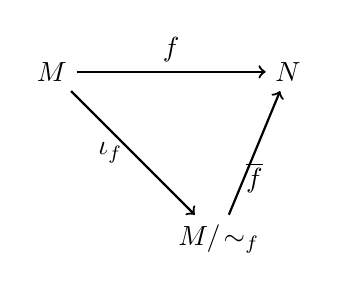
\begin{tikzpicture}[node distance=3cm, auto]
		\node (M) {\(M\)};
		\node (N) [right of=M] {\(N\)};
		\node (Mquot) [below right of=M] {\(M/\!\sim_f\)};
		
		\draw[->, thick] (M) -- node[above] {\(f\)} (N);
		\draw[->, thick] (M) -- node[left] {\(\iota_f\)} (Mquot);
		\draw[->, thick] (Mquot) -- node[below] {\(\overline{f}\)} (N);
		
	\end{tikzpicture}
	\label{fig:homomorphism_theorem}
\end{figure}

This is saying us to first form collections of elements and then use our second function to associate that connections to their 
respective images. 

\subsection{Representatives}

Given a set \(X \subseteq A\), we consider it a set of \emph{representatives} for a partition \(S\) if 

\[
	\forall Y \in S X \cap Y = \{a\}, a \in A
\]

\subsection{Family of Subsets Operations}

Let \(\mathscr{F}\) be a system of sets (a family of subsets) on the set \(X\). We define:

\[
	\bigcup_{M \in F} M := \bigcup F := \{ x \in X : \text{there exists } M \in F \text{ such that } x 
	\in M \} ,
\]

\[
	\bigcap_{M \in F} M := \bigcap F := \{ x \in X : x \in M \text{ for all } M \in F \} .
\]


\subsection{Product of Classes}

Given a family of classes \(\{A_i\}_{i \in I}\) we define the \emph{product of classes} as 

\[
	\prod A_i = \{f: I \to A \mid f(i) \in A_i \land i \in I\}
\]

Is the set of all functions from \(I\) to \(\bigcup A_i\).

\subsubsection*{Properties}

\begin{itemize}

	\item \(\left(\prod_{i \in I} A_i\right) \cap \left(\prod_{j \in J} B_j\right) = \prod_{(i, j) \in I \times J}(A_i \cap B_i)\)
	
	\item \(\left(\prod_{i \in I} A_i\right) \cup \left(\prod_{j \in J} B_j\right) = \prod_{(i, j) \in I \times J}(A_i \cup B_i)\)	

\end{itemize}

\subsection{Pigeon Principle}

For \(g: A \to B\) and \(|A| = n + 1\), \(|B| = n\) then there exists \(b \in B\) such that \(|g^{-1}(\{ b \})| \ge 2\). 

In other words if you have \(n\) boxes and \(n + 1\) objects, then at least one of those boxes will have more than 2 elements.

\subsection{The Cantor Set}

In the following, we want to study the Cantor set \(\mathcal{C}\subseteq\R\).

First, we describe its construction informally: We start with the unit interval \(A_0:=[0,1]\) and remove from it the "middle third" (where the boundary points are not removed).
The result \(A_1\) thus consists of the sub-intervals \(\left[0,\frac{1}{3}\right]\) and \(\left[\frac{2}{3},1\right]\). 
Now we remove from each of these two sub-intervals the middle third and continue in this manner.

For fixed but arbitrary \(n\in\N_0\), \(A_n\) thus consists of \(2^n\) pairwise disjoint closed sub-intervals of length \(3^{-n}\), 
and \(A_{n+1}\) arises from \(A_n\) by removing the middle third from each of these sub-intervals. What "remains" is the Cantor set.

Now mathematically precise: For \(n\in\N_0\), let 

\[
	A_{n+1}:=\frac{A_n}{3} \cup (\frac{2+A_n}{3}), \text{ with } A_0 = [0,1]
\]
	
Regarding the notation - for \(X\subseteq\R\) and \(a,t\in\R\), we define

\[
    aX:=\{ax:x\in X\}
\]

\[
    t+X:=\{t+x:x\in X\}
\]

Then \(\mathcal{C}:=\bigcap_{n=0}^\infty A_n\).

For the intuition, imagine our fraction squishing all the numbers and then adding two to a copy of those numbers. Then repeating 
the process multiple times.

\textbf{Properties:}

\begin{itemize}

	\item The Cantor Set is uncountable 
	
	\item The Cantor Set has a length of 0 
	
	\item The set can be interpreted as all infinite sequences of zeroes and ones, when handling left and right as 0 and one.

\end{itemize}

\textbf{Proof I:}
We give a proof by contradiction.

Assume the Cantor set is countable. Then there exists a surjective function

\[
	c : \N \to \mathcal{C}.
\]

After the first step of the Cantor construction we have

\[
	A_{1} = [0,\tfrac{1}{3}] \cup [\tfrac{2}{3}, 1].
\]

Since

\[
	c(1) \in \mathcal{C} \subset A_{1},
\]

the point \(c(1)\) lies in exactly one of the two disjoint intervals.  
We choose the other interval and call it \(I_{1}\).

Thus:

\begin{itemize}

	\item \(I_{1} \subset A_{1}\),

	\item \(I_{1}\) is closed,

	\item \(c(1) \notin I_{1}\).

\end{itemize}


For the inductive step, assume there exists a closed interval

\[
	I_{n} \subset A_{n} \quad \text{with} \quad c(n) \notin I_{n}.
\]

When passing from \(A_{n}\) to \(A_{n+1}\), the middle third of each interval is removed.
Therefore, \(I_{n}\) splits into exactly two disjoint closed sub-intervals of \(A_{n+1}\).

Since \(c(n+1)\) can lie in only one of these two intervals, we choose the other and call it \(I_{n+1}\).

Thus:

\begin{itemize}

	\item \(I_{n+1} \subsetneq I_{n}\),

	\item \(I_{n+1}\) is closed and non-empty,

	\item \(c(n+1) \notin I_{n+1}\).

\end{itemize}


By construction the nested sequence

\[
	I_{1} \supsetneq I_{2} \supsetneq I_{3} \supsetneq \cdots
\]

is obtained, and the lengths satisfy

\[
	|I_{n}| = 3^{-n}.
\]

Thus, the lengths converge to \(0\).


Since the intervals are closed, bounded, nested, and their lengths tend to \(0\), the interval-nesting principle implies:

\[
	\bigcap_{n=1}^{\infty} I_{n} \neq \varnothing.
\]

There exists exactly one point

\[
	x \in \bigcap_{n=1}^{\infty} I_{n}.
\]

Since each \(I_{n} \subset A_{n}\), it follows that

\[
	x \in \mathcal{C}.
\]

\subsection*{Contradiction}

Because \(c\) is surjective by assumption, there exists a \(k \in \N\) such that

\[
	x = c(k).
\]

However, by our construction \(I_{k}\) was chosen so that

\[
	c(k) \notin I_{k},
\]

while at the same time

\[
	x \in I_{k}.
\]

This is a contradiction. Thus, the assumption that the Cantor set is countable leads to a contradiction.
Therefore, the Cantor set has to be uncountable.

\QED 

\textbf{Proof II:}

This is not the most rigorous proof, but accomplishes its goal:

The original interval as length 1 and consist of one unit, the next \(1 - \frac{1}{3}\) and consist of two units, this pattern with 
\(2^n \frac{1}{3^n}\) continues forever thus, 

\[
	L = 1 - \sum_{i = 1}^{\infty} 2^n \frac{1}{3^n}
\]

Note that the sum is a geometric series therefore, 

\[
	L = 1 - 1 = 0
\]

\QED


